\documentclass[11pt,twoside]{article}

\usepackage{amsmath}
\usepackage{amssymb}
\usepackage{amsthm}
\usepackage{courier} % Required for the courier font
\usepackage{extramarks} % Required for headers and footers
\usepackage{fancyhdr} % Required for custom headers
\usepackage{graphicx} % Required to insert images
\usepackage{lastpage} % Required to determine the last page for the footer
\usepackage{listings} % Required for insertion of code
\usepackage{lipsum} % Used for inserting dummy 'Lorem ipsum' text into the template
\usepackage{mathtools}
\usepackage{subcaption}

\usepackage[margin=1in]{geometry}
\usepackage[usenames,dvipsnames]{color} % Required for custom colors

\begin{document}

\title{CSC411 - Project \#4}
\author{Yui Chit (Michael) Wong - 999806232\\Yijin (Catherine) Wang - 998350476}
\maketitle

\clearpage

\section*{Part 1}
\paragraph{Question}
Explain precisely why the code corresponds to the pseudocode below. Specifically, in your report, explain how all the terms ( $G_t$ , $\pi$ , and the update to $\theta$ ) are computed, quoting the relevant lines of Python.

\begin{figure*}[h]
	\centering
	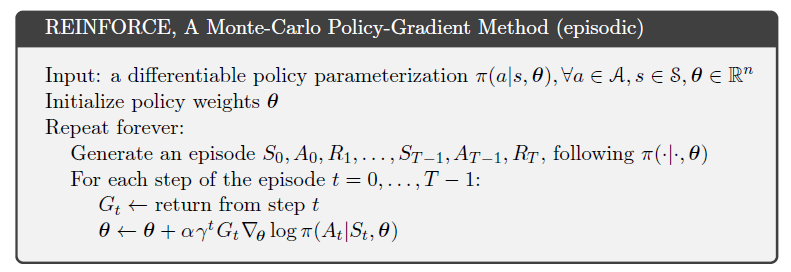
\includegraphics[scale=0.8]{sutton&barto.png}
	\caption*{Pseudocode}
\end{figure*}

\paragraph{Answer}
As mentioned on the assignment page, the policy function $\pi_{\theta}$ is implemented with a single-hidden-layer of neural network. Since the actions for the bipedal walker is continuous, we have to use a Gaussian distribution on $\pi$. Thus we pass the hidden layer into two separately fully connected output, which represents the $\mu$ and $\sigma$ to the normal distribution. The activation function are $tanh$ and $softplus$ (variation on $ReLU$) respectively. The $sigma$ value are also clipped if it is too small or big.

\begin{figure*}[h]
	\centering
	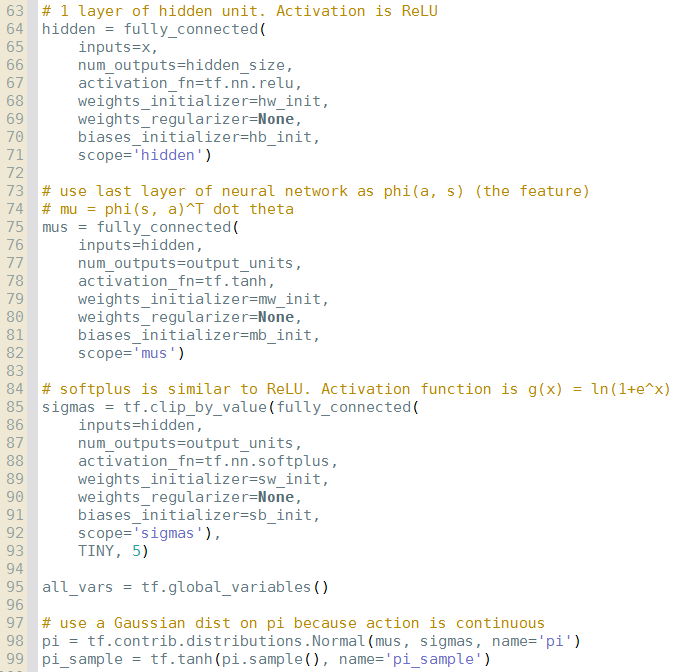
\includegraphics[scale=0.8]{part1_mu&sigma.png}
	\caption*{Generating distribution on $\pi$}
\end{figure*}

As for the weight intialization, if there is no weight saved from the previous run, we will initialize the weight $\theta$. There are one $w$ and $b$ for each of the layers (hidden, $\mu$, $\sigma$). When initializing the weight to each layer, the program uses $xavier initialization$, another variation of random weight initialization that keep the scale of the gradients in roughly the same scale.

\begin{figure*}[h]
	\centering
	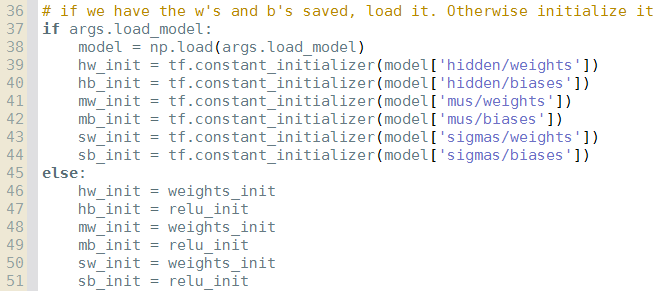
\includegraphics[scale=0.8]{part1_weight_init.png}
	\caption*{Weight ($\theta$) initialization}
\end{figure*}

Once everything is initialized, we will start training. For each iteration, we will reset the environment (line 118), then generate the states, actions, and rewards from time 0 to time $T$. When generating the actions, we will randomly sample a $\pi_{sample}$ from the $\pi$ normal distribution (line 133-135). Then based on the $\pi_{sample}$, we will generate the corresponding action, and using the action, the new state, reward would be generated. We will keep track of all the states, actions, and rewards in 3 lists ($ep_states, ep_actions, $ and $ep_rewards$). We will also keep track of the total discounted rewards using the variable $G$ (line 137). Then to obtain $G_t$, the discounted reward starting from time t, the program calls a culmulation sum function on the $ep_rewards$ then subtract it from $G$ (line 148). Thus $returns$ would be storing the total discouned rewards for each time from time 0 to $T-1$.

\begin{figure*}[h]
	\centering
	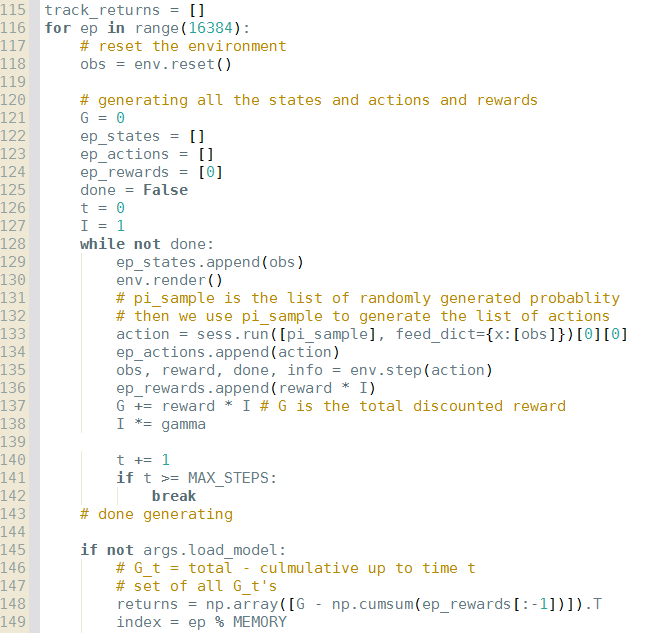
\includegraphics[scale=0.8]{part1_generate.png}
	\caption*{States, actions, and rewards generation based on $\pi_{sample}$}
\end{figure*}

Then we will pass the list of states, actions, and the returns into the training step (line 154-157). Then tensorflow will use the state and the weights to generate a new $\mu$ and $\sigma$ (line 63-93). Then it will compute the log probability of the actions given the generate $\mu$ and $\sigma$ (line 102). The cost function used is $J(\theta) = -\sum[G_t log \pi (A_t | S_t, \theta)]$. The program uses gradient descent to adjust the $\theta$ to minimize the cost function (line 105-107).

\clearpage



\section*{Part 2}

\paragraph{Question}

\paragraph{Answer}

\clearpage



\section*{Part 3}

\paragraph{Question}

\paragraph{Answer}

\clearpage



\end{document}